Tratar as metodologias e abordagens por partes será a melhor abordagem para analisar os resultados e gerar discussões de forma mais clara e coesa.

A primeira parte a ser analisada é a mineração de dados. No final foram obtidos 21 perfis, de 907 tweets negativos, desses 310 continham uma ou mais questões da EADS ligadas a ele, contabilizando um total de 688 questões respondidas. Representando assim 34\% dos tweets negativos tendo em média 2.2 questões da EADS relacionadas a ele.

Sobre a mineração alguns pontos e conclusões podem ser retirados. A primeira é a falta de outras "rodadas" de coleta e mineração com outros conjuntos de palavras chaves poderiam ter feito a diferença, uma vez que o corpo de perguntas menos respondidas são conhecidos, uma mineração envolvendo um aumento desse tipo de tweet poderia nivelar a base de conhecimento. E por fim se a falta de profissionais da psicologia/psiquiatria dentro do projeto. Com conhecimento mais sólido e tempo seriá capaz mapear, em caso de não localizar, frases que contemplassem as questões com menos dados, podendo assim, preencher o banco de dados manualmente. Além disso, com um grupo maior de profissionais a chance das respostas serem mais apropriadas aumentam, sem contar o fato de uma quantidade maior de profissionais poderia dar conta de analisar "rodadas" de mineração cada vez maiores.

A segunda parte implica sobre o modelo de predicção de questões EADS. Por mais acertividade que algo com poucos dados tenha conquistado o \textit{score} do modelo aplicando Naive Bayes foi de 42\%, onde já foi evidenciado que a falha nos \textit{recalls} esta atrelado com a falta de dados. Ao observar a Figura \ref{fig:rpr} pode-se notar a relação inversa de precisão e recuo perante a quantidade de tweets classificados. Quanto maior a quantidade de tweets maior a precisão e menor a taxa de recuo.

\begin{figure}[!ht]
    \centering
    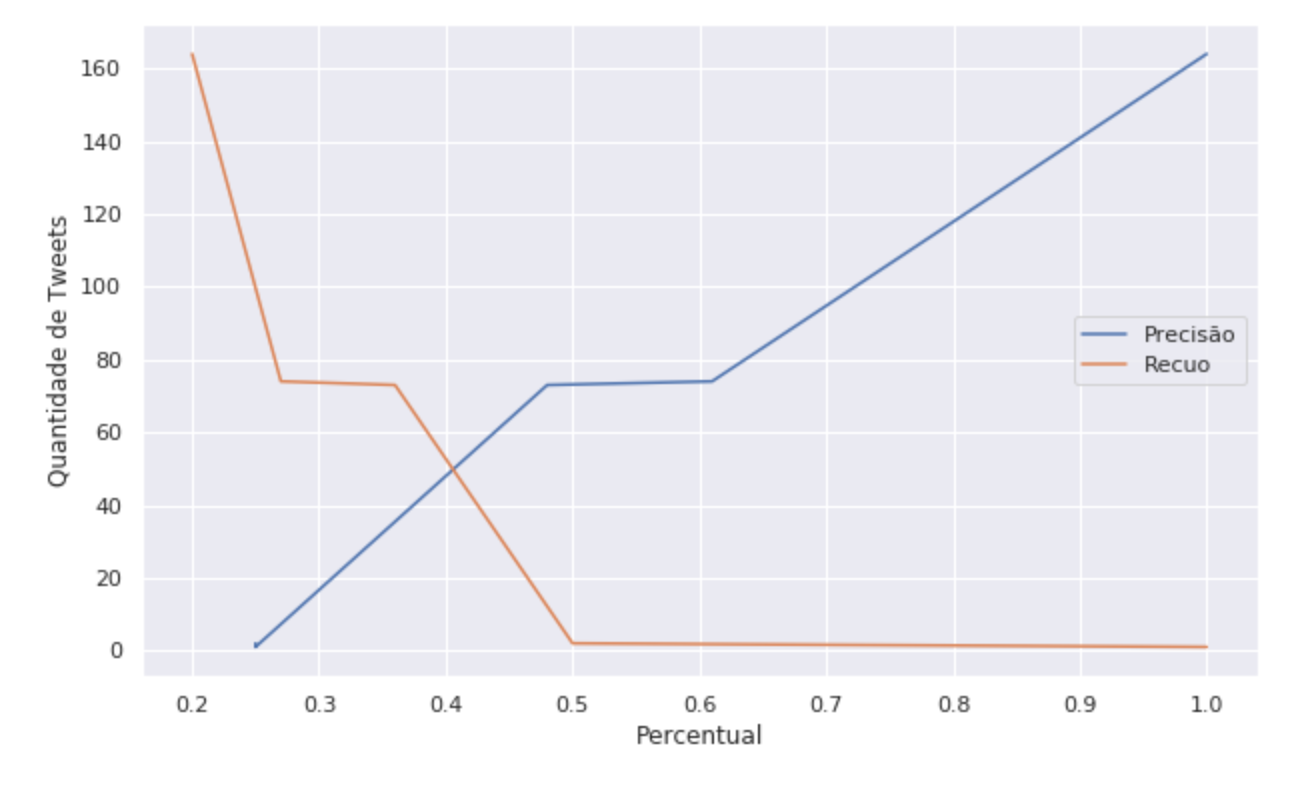
\includegraphics[width=.75\textwidth]{imagens/rpr.png}
    \caption{Relação de sentimentos por tweet dentro da massa de dados}
    \label{fig:rpr}
\end{figure}

Entretanto, na Figura \ref{fig:qpp} pode-se notar que a pontuação não segue esse padrão. Por determinado motivo a taxa de melhor conversão, relacionando os gráficos, seria entre 60 a 80 tweets. Porém, o questionamento fica explicitado, o melhor resultado viria de um banco mais heterogeneo, onde todas as perguntas tivessem média de 60 a 80 tweets classificados.

\begin{figure}[!ht]
    \centering
    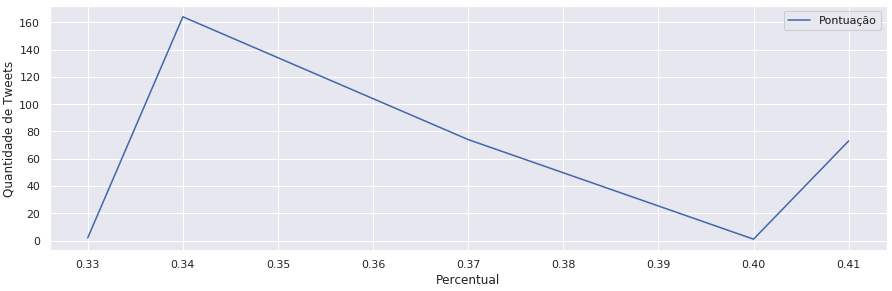
\includegraphics[width=.8\textwidth]{imagens/qpp.png}
    \caption{Relação de sentimentos por tweet dentro da massa de dados}
    \label{fig:qpp}
\end{figure}

Logo, ter muitos dados seria algo relativo, o importante em fato, seria ter uma quantidade plausivel de dados em cada item, sem uma divergencia muito grande, como acontece principalmente com o a questão "Não tive nenhum sentimento positivo". Para evidenciar isso e partindo da premissa que primeira análise que gerou os gráficos a partir dos tweets minerados para o cenário, foi gerada uma segunda predicção adicionando na massa os dados coletados dos usuários na segunda parte da pesquisa. Aumentando assim a quantidade de itens de aproximadamente 690 para aproximadamente 1100 repostas. Se acompanhar a Figura \ref{fig:prediction2} é possível notar uma queda no \textit{score}, o que indica que uma base com dados pareados tende a ser mais efetiva do que uma base com muitos dados dispersos. Vale lembrar que a divergencia das questões pode vir a ser um problema de falta de dado especialista. Uma vez que os dados utilizados foram inseridos a partir do conhecimento teórico do autor com ajuda de algumas das biografia citadas préviamente na pesquisa.

\begin{figure}[!ht]
    \centering
    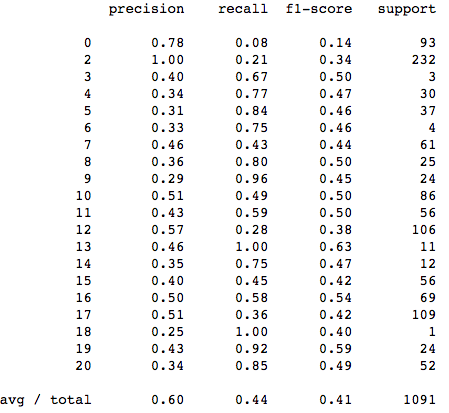
\includegraphics[width=.5\textwidth]{imagens/prediction2.png}
    \caption{Tabela de resultados do Naive Bayes para 1091 resultados}
    \label{fig:prediction2}
\end{figure}

Por fim, para inferir a EADS em si, é necessário recorrencia, em outras palavras, inferir um item é apenas uma parte do processo, a escala é feita semanalmente, logo uma pergunta isolada pode ter menos representatividade do que uma pergunta que aparece recorrentemente em um periodo de tempo. A falta de dados não permite que afirmações especificas relacionadas ao modelo sejam feitas, entretanto, é possível dizer que existe relação entre a expressão de um perfil no Twitter ao seu estado emocional, logo é possível, inferir a EADS utilizando recursos da inteligencia artificial. Se em um caso de poucos recursos e dados foi possível obter uma pontuação de 42\%, em um cenário melhor pesquisas futuras podem chegar a acertos de 70\% a 80\%, igualando hoje com pesquisas similares que unicamente classificão publicações como depressivas, o que de certo modo não contempla toda a complexidade da pesquisa apresentada até então.